\documentclass[12pt,a4paper]{article}

\usepackage[a4paper,top=2cm,bottom=2cm,left=2.5cm,right=1cm]{geometry}
\usepackage[T2A]{fontenc}
\usepackage[utf8]{inputenc}
\usepackage[russian]{babel}
\usepackage{mathptmx}




\usepackage{graphicx}
\graphicspath{{/mnt/data/}}
\usepackage{booktabs}
\usepackage{array}
\usepackage{float}
\usepackage{amsmath}
\usepackage{titlesec}
\usepackage{fancyhdr}
\usepackage{setspace}
\usepackage{ragged2e}

\setlength{\parindent}{1cm}
\setlength{\parskip}{0pt}
\onehalfspacing
\justifying
\sloppy

\titleformat{\section}{\bfseries\fontsize{14}{16}\selectfont}{\thesection}{0.6em}{}
\titleformat{\subsection}{\bfseries\fontsize{12}{14}\selectfont}{\thesubsection}{0.6em}{}
\titlespacing*{\section}{0pt}{12pt}{6pt}
\titlespacing*{\subsection}{0pt}{10pt}{4pt}

\pagestyle{fancy}
\fancyhf{}
\fancyfoot[R]{\thepage}
\renewcommand{\headrulewidth}{0pt}
\renewcommand{\footrulewidth}{0pt}

\begin{document}

\begin{titlepage}
\thispagestyle{empty}
\begin{center}
НОВОСИБИРСКИЙ ГОСУДАРСТВЕННЫЙ УНИВЕРСИТЕТ

\vspace{0.5cm}
Механико-математический факультет\\
Цифровые двойники и научный инжиниринг
\end{center}

\vspace{1.5cm}
\begin{flushleft}
ОТЧЁТ ПРИНЯТ\\
Оценка \underline{\hspace{4cm}}\\
\underline{\hspace{2cm}} / \underline{\hspace{3cm}} /\\
«\underline{\hspace{0.8cm}}» \underline{\hspace{3cm}} 2026 г.
\end{flushleft}

\vfill
\begin{center}
{\bfseries ОТЧЁТ}\\[0.6cm]
по лабораторной работе № 1\\[0.3cm]
«Параллельные циклы»\\[0.3cm]
по дисциплине «Параллельное программирование»
\end{center}

\vfill
\begin{flushright}
Студент гр. 25157\\
Ф.И.О. Заволокина Варвара Антоновна
\end{flushright}

\vfill
\begin{center}
Новосибирск -- 2026
\end{center}
\end{titlepage}

\setcounter{page}{2}

\section{Постановка задачи}

\subsection{Цель работы}

Цель работы -- знакомство со спецификацией OpenMP, освоение распараллеливания циклов, управления числом потоков, использования разделяемых и частных переменных, редукции, критических секций и политик планирования итераций.

В ходе лабораторной работы требовалось выполнить примеры из методического пособия, исследовать ошибочные ситуации при некорректной работе с общими данными, а также разработать и исследовать параллельную программу по индивидуальному варианту. В качестве индивидуального задания выбрано построение изображения множества Мандельброта.

\subsection{Теоретические сведения}

OpenMP -- прикладной программный интерфейс для организации параллельных вычислений в системах с общей памятью. Параллельное выполнение строится по модели fork-join: начальный поток создаёт команду потоков при входе в параллельную область, после чего потоки совместно выполняют работу и синхронизируются при завершении области.

Для распределения независимых итераций цикла использовалась директива \texttt{\#pragma omp parallel for}. Она позволяет автоматически разделить итерации между потоками команды.

Для безопасного суммирования результатов применялась опция \texttt{reduction(+:sum)}, при которой каждый поток получает локальную копию переменной, а частичные результаты объединяются после выполнения параллельной области.

Переменные OpenMP делятся на разделяемые и частные. Разделяемая переменная доступна всем потокам через одну область памяти. Частная переменная имеет отдельную копию в каждом потоке. Некорректный одновременный доступ нескольких потоков к разделяемой переменной без синхронизации приводит к гонке данных.

Директива \texttt{\#pragma omp critical} ограничивает выполнение следующего участка: одновременно его может выполнять только один поток. Такой подход обеспечивает корректность, но может снижать производительность из-за последовательного доступа к критической секции.

Опция \texttt{schedule} определяет порядок выдачи итераций потокам. При \texttt{static} распределение выполняется заранее крупными непрерывными блоками. При \texttt{dynamic} поток получает новые блоки итераций по мере завершения предыдущих. Динамическая политика полезна при неоднородной трудоёмкости отдельных итераций.

\section{Разработка решения}

\subsection{Проверка работы OpenMP}

Работа начата с компиляции и запуска примера 19. На macOS системный Apple Clang не обнаруживал заголовочный файл \texttt{omp.h}, поэтому для лабораторной использован GCC 16.2.0, установленный через Homebrew. Сборка OpenMP-программ выполнялась компилятором \texttt{g++-16} с ключом \texttt{-fopenmp}. Для доступа к системным заголовочным файлам macOS дополнительно передавался путь к SDK через \texttt{-isysroot}.

Типовая команда сборки:

\begin{verbatim}
g++-16 -isysroot "$(xcrun --show-sdk-path)" -O3 -fopenmp file.cpp -o file
\end{verbatim}

Для исследования загрузки процессора пример 19 был модифицирован: присваивание заменено вызовом чистой вычислительно тяжёлой функции. При последовательной сборке время выполнения составило 2.608 с, а при использовании OpenMP время уменьшалось с ростом числа потоков.

\begin{table}[H]
\centering
\caption{Время выполнения модифицированного примера 19}
\begin{tabular}{cccc}
\toprule
Число потоков & Время, с & CPU, \% & Ускорение \\
\midrule
1 & 2.571 & 99  & 1.00 \\
2 & 1.332 & 198 & 1.93 \\
3 & 0.920 & 287 & 2.79 \\
4 & 0.685 & 390 & 3.75 \\
\bottomrule
\end{tabular}
\end{table}

\subsection{Эксперименты с общими данными и синхронизацией}

В примере суммирования массива корректная версия с \texttt{reduction} для массива от 0 до 99 стабильно возвращала значение 4950. После удаления \texttt{reduction} переменная \texttt{sum} стала разделяемой и изменялась потоками без синхронизации. В серии запусков наблюдались как случайно корректные значения, так и ошибочные результаты 3531 и 4355. Это подтверждает недетерминированный характер гонки данных.

Отдельно исследовано вынесение переменной \texttt{id} из класса \texttt{private} в класс \texttt{shared}. Порядок вывода сообщений потоков стал непредсказуемым, строки перемешивались. Даже если отдельный запуск визуально показывает допустимые номера потоков, программа содержит гонку данных и её поведение не гарантируется спецификацией.

Затем пример суммирования был переписан без \texttt{reduction} с использованием \texttt{critical}. Итоговая сумма снова стала равна 4950, то есть критическая секция обеспечивает корректность. При этом \texttt{reduction} предпочтительнее для суммирования, так как позволяет выполнять накопление локально в каждом потоке и уменьшает число точек взаимного исключения.

\subsection{Индивидуальное задание: множество Мандельброта}

Для каждой точки комплексной плоскости $c$ выполняется итерационный процесс
\[
z_0 = 0, \qquad z_{n+1}=z_n^2+c.
\]
Если модуль $z$ превышает 2, считается, что последовательность расходится. Число итераций до выхода используется для определения яркости пикселя. Для точек внутри множества достигается установленный предел числа итераций.

Расчёт каждого пикселя независим от остальных, поэтому задача естественно распараллеливается по строкам изображения. Однако трудоёмкость строк неодинакова: точки вне множества могут завершать итерации быстро, тогда как точки внутри или вблизи границы требуют существенно большего числа итераций.

В последовательной версии значение каждого пикселя сразу записывалось в PPM-файл. В параллельной версии запись из рабочих потоков была исключена: сначала каждый поток заполнял независимые элементы общего массива \texttt{pixels}, после завершения вычислений файл формировался последовательно. Это устраняет гонку при работе с потоком вывода и позволяет отдельно измерять именно вычислительную часть.

Для измерения времени вычислительного цикла использовалась функция \texttt{omp\_get\_wtime()}, а запись PPM-файла в измеряемый интервал не включалась.

\section{Результаты экспериментов}

\subsection{Вычислительная среда и методика измерений}

Эксперименты выполнены на ноутбуке MacBook Pro под управлением macOS. Среда разработки -- Visual Studio Code. Компилятор -- GNU g++ 16.2.0 (Homebrew) с поддержкой OpenMP. Точная модель процессора: Chip: Apple M2 Pro, Total Number of Cores: 10 (6 performance and 4 efficiency), Memory: 16 GB. Исследовалось выполнение с 1, 2, 4 и 8 OpenMP-потоками.

Производительность индивидуального задания измерялась непосредственно вокруг параллельного вычислительного цикла функцией \texttt{omp\_get\_wtime()}. Для каждой конфигурации выполнено по три запуска; в таблицах приведены отдельные значения и среднее арифметическое. Запись изображения на диск исключалась из измеряемого времени.

Корректность проверялась сравнением SHA-хешей выходных PPM-файлов последовательной и параллельной версий, а также запуском параллельной версии с различным количеством потоков.

\subsection{Проверка корректности}

Для последовательного файла \texttt{mandelbrot.ppm} и параллельного файла \texttt{mandelbrot\_omp.ppm} получен одинаковый SHA-1:

\begin{center}
\texttt{67d7869e01743b3256edf0e3a4138d1bed72c55a}
\end{center}

Тот же хеш сохранялся при запусках параллельной программы с 1, 2, 4 и 8 потоками. Следовательно, число потоков и выбранная политика планирования не изменяют вычисляемое изображение.

\subsection{Производительность static и dynamic}

\begin{table}[H]
\centering
\caption{Повторные измерения времени вычисления множества Мандельброта}
\small
\begin{tabular}{ccrrrr}
\toprule
Политика & Потоки & Запуск 1, с & Запуск 2, с & Запуск 3, с & Среднее, с \\
\midrule
static  & 1 & 0.609872 & 0.599140 & 0.600135 & 0.603049 \\
static  & 2 & 0.321917 & 0.309735 & 0.309761 & 0.313804 \\
static  & 4 & 0.303939 & 0.316452 & 0.302860 & 0.307750 \\
static  & 8 & 0.211124 & 0.211540 & 0.211577 & 0.211414 \\
\midrule
dynamic & 1 & 0.610500 & 0.598327 & 0.609372 & 0.606066 \\
dynamic & 2 & 0.310766 & 0.309373 & 0.311315 & 0.310485 \\
dynamic & 4 & 0.158423 & 0.158461 & 0.158767 & 0.158550 \\
dynamic & 8 & 0.096201 & 0.095401 & 0.094740 & 0.095447 \\
\bottomrule
\end{tabular}
\end{table}

Ускорение вычислялось по формуле
\[
S_p=\frac{T_1}{T_p},
\]
а эффективность -- по формуле
\[
E_p=\frac{S_p}{p},
\]
где $T_1$ -- среднее время на одном потоке, $T_p$ -- среднее время на $p$ потоках.

\begin{table}[H]
\centering
\caption{Ускорение и эффективность параллельной реализации}
\begin{tabular}{ccccc}
\toprule
Политика & Потоки & Среднее время, с & $S_p$ & $E_p$ \\
\midrule
static  & 1 & 0.603049 & 1.00 & 1.00 \\
static  & 2 & 0.313804 & 1.92 & 0.96 \\
static  & 4 & 0.307750 & 1.96 & 0.49 \\
static  & 8 & 0.211414 & 2.85 & 0.36 \\
\midrule
dynamic & 1 & 0.606066 & 1.00 & 1.00 \\
dynamic & 2 & 0.310485 & 1.95 & 0.98 \\
dynamic & 4 & 0.158550 & 3.82 & 0.96 \\
dynamic & 8 & 0.095447 & 6.35 & 0.79 \\
\bottomrule
\end{tabular}
\end{table}

\begin{figure}[H]
\centering
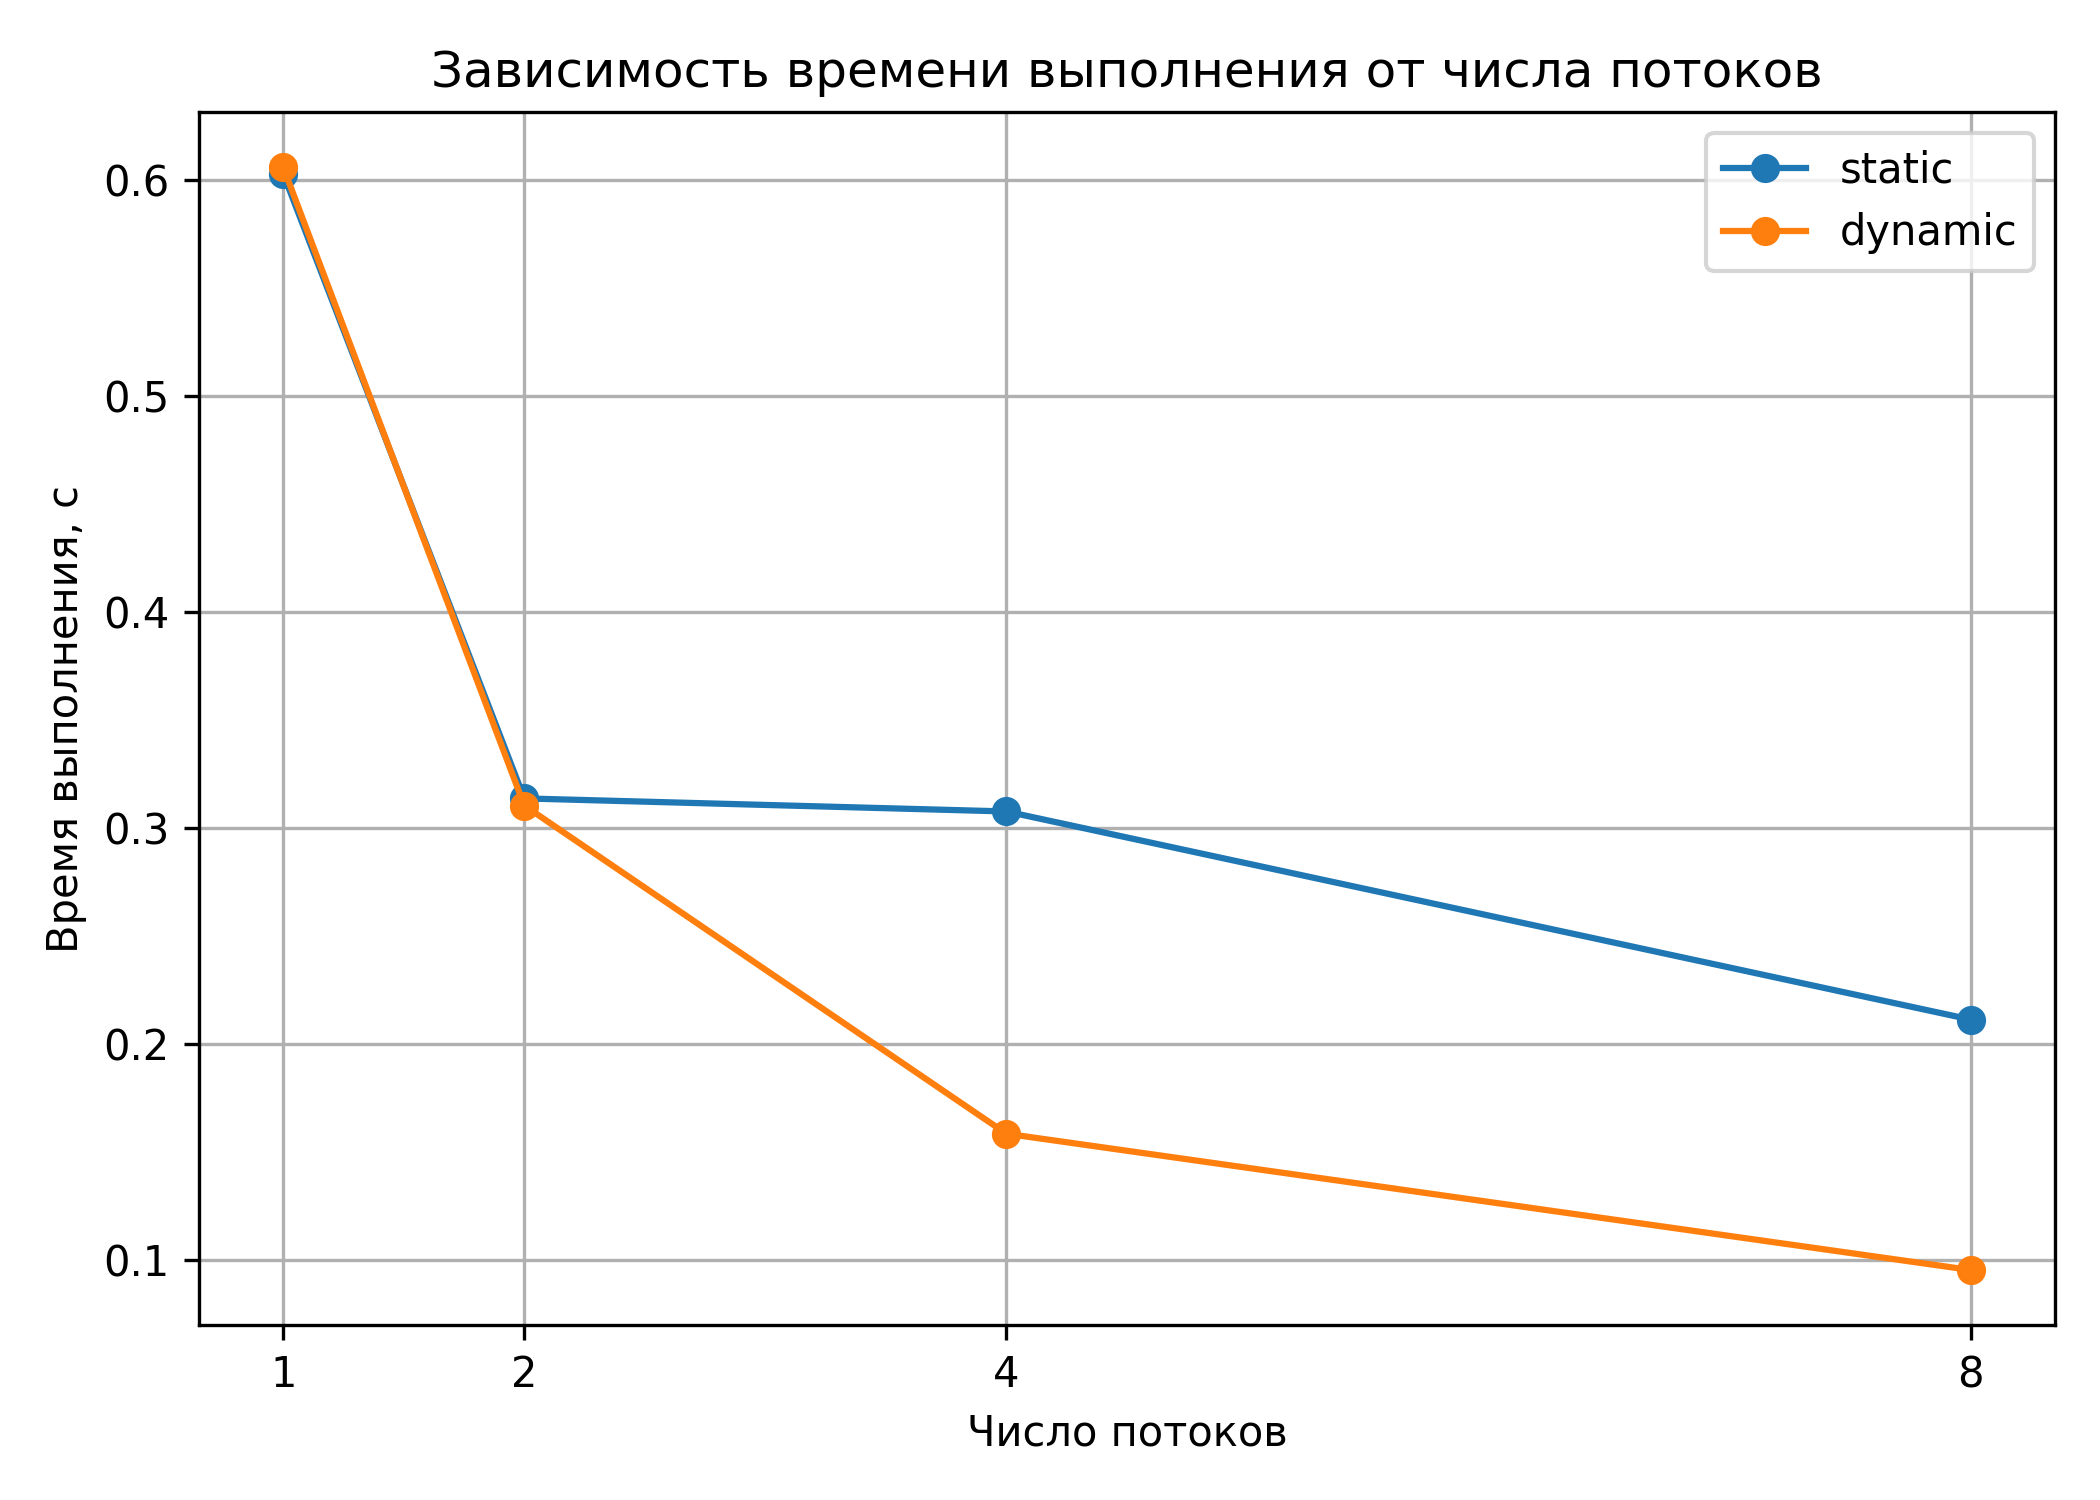
\includegraphics[width=0.72\textwidth]{time_vs_threads.png}
\caption{Зависимость среднего времени вычисления от числа потоков}
\end{figure}

\begin{figure}[H]
\centering
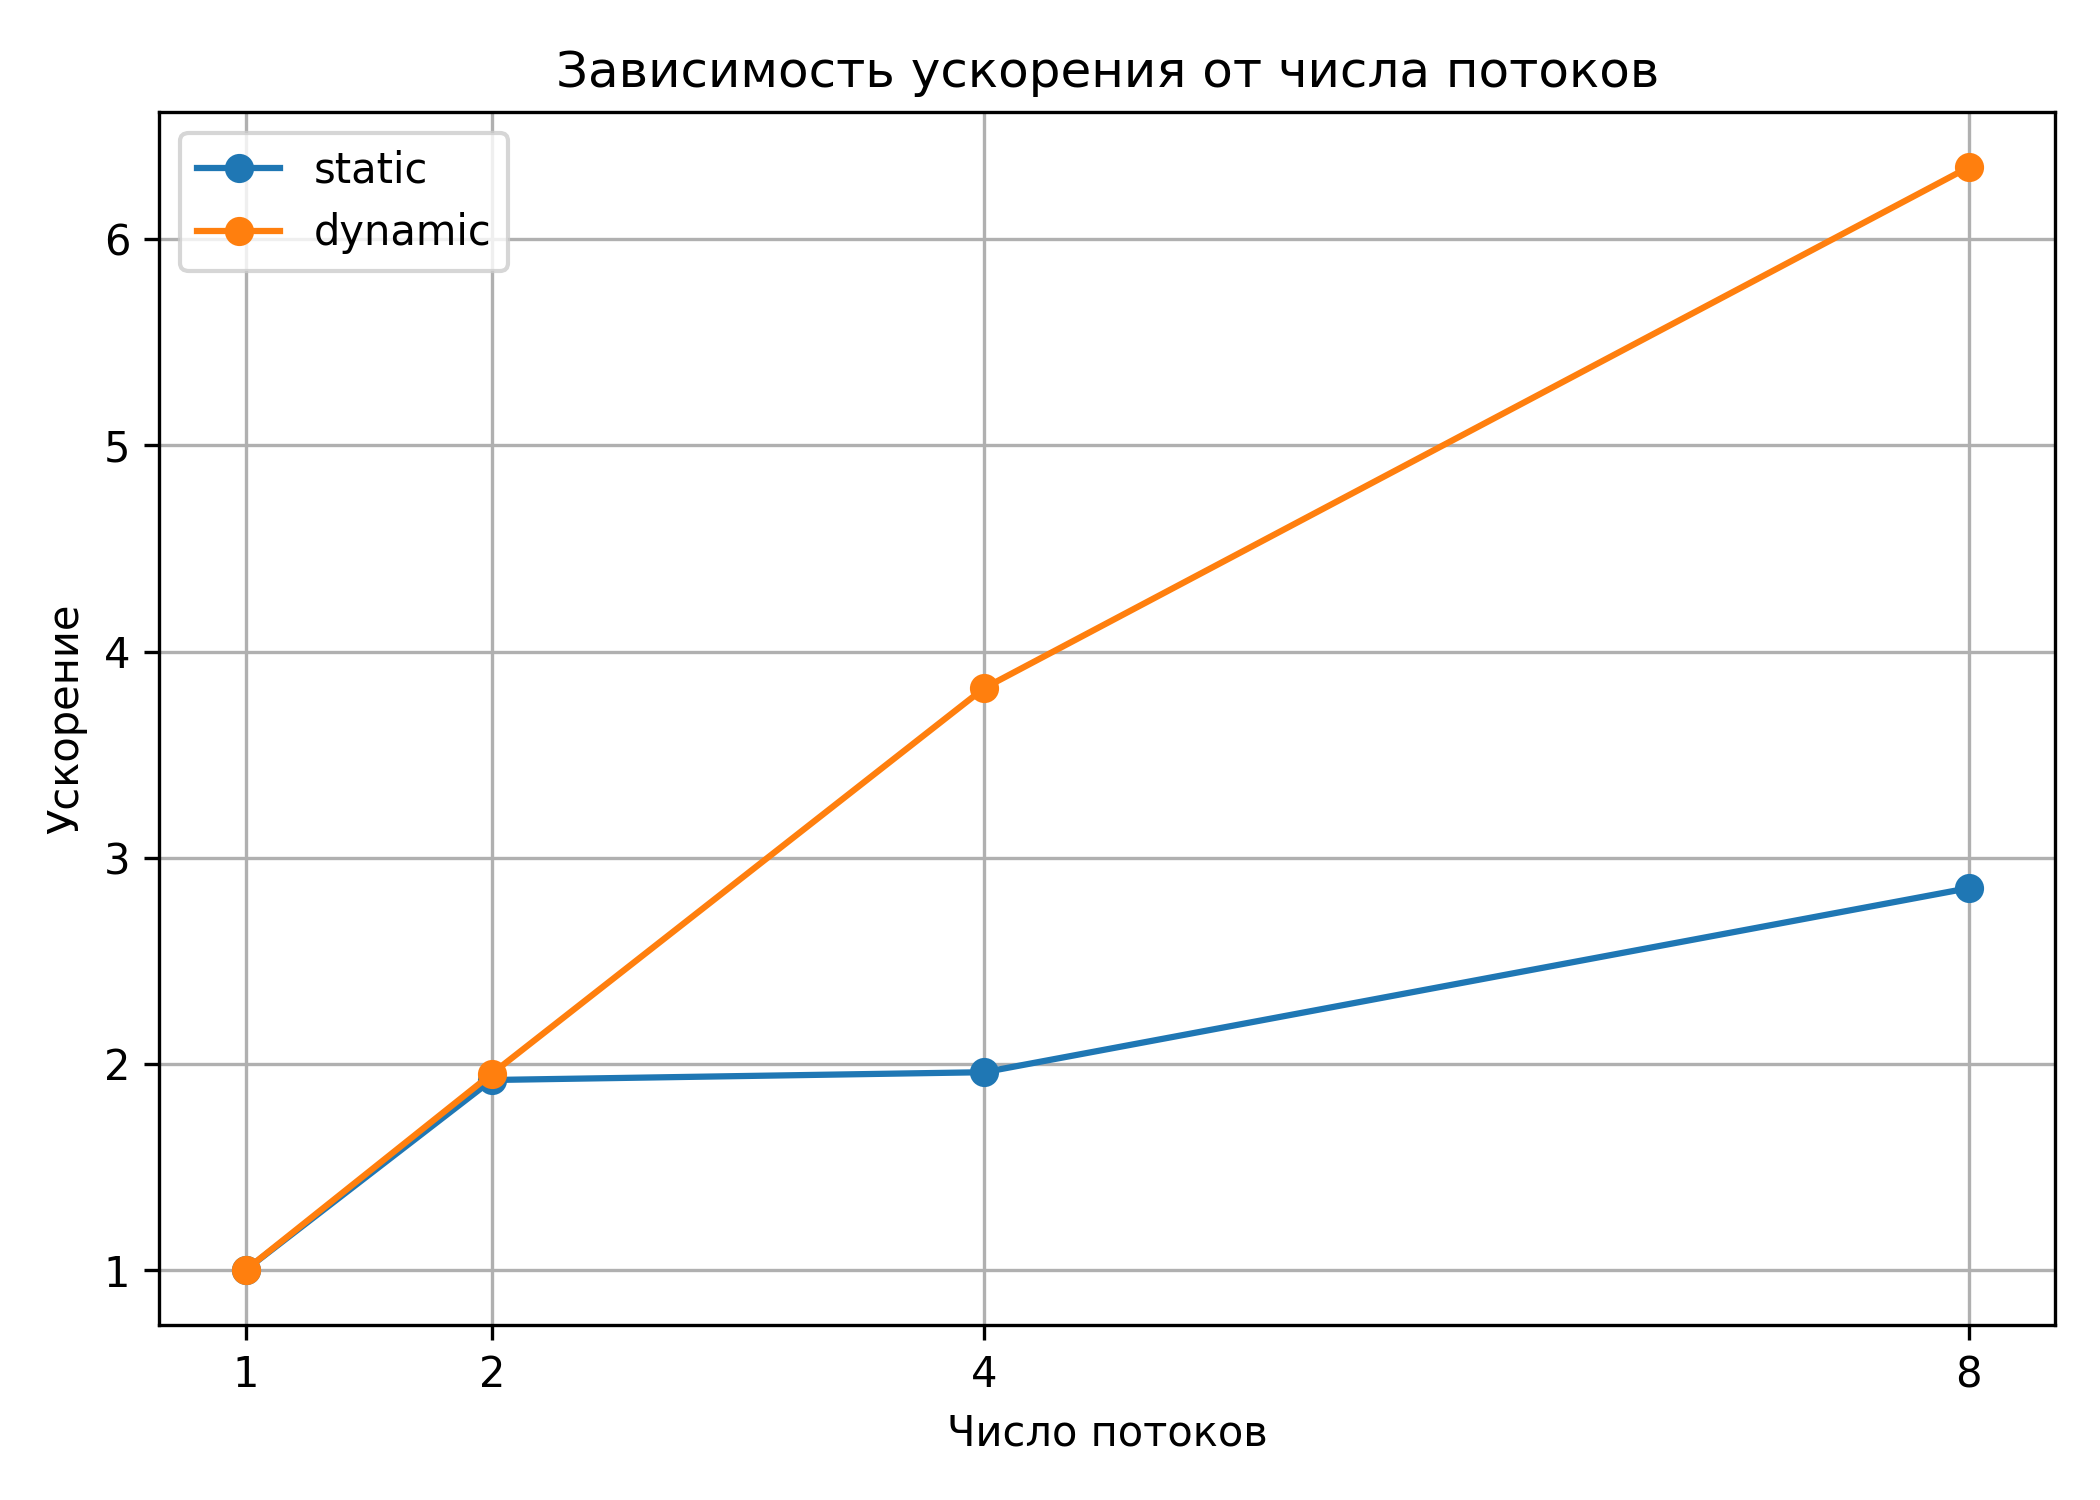
\includegraphics[width=0.72\textwidth]{speedup_vs_threads.png}
\caption{Ускорение параллельной реализации}
\end{figure}

\subsection{Анализ результатов}

При одном и двух потоках \texttt{static} и \texttt{dynamic} дают практически одинаковое время: около 0.60 с и 0.31 с соответственно. При дальнейшем увеличении числа потоков различия становятся значительными.

Для \texttt{dynamic} при четырёх потоках среднее время равно 0.158550 с, ускорение -- 3.82, эффективность -- 0.96. При восьми потоках время уменьшается до 0.095447 с, ускорение достигает 6.35, а эффективность составляет 0.79. Это указывает на хорошую балансировку нагрузки и относительно небольшие накладные расходы.

Для \texttt{static} при четырёх потоках время составляет 0.307750 с, то есть почти не улучшается относительно двух потоков. Ускорение равно 1.96, эффективность -- 0.49. При восьми потоках ускорение возрастает до 2.85, но эффективность остаётся низкой -- 0.36.

Причина различия связана с неодинаковой вычислительной сложностью строк изображения. При \texttt{static} крупные непрерывные блоки строк закрепляются за потоками заранее. Поток, получивший строки с большим количеством точек внутри и около границы множества, выполняет существенно больше итераций, тогда как другие потоки завершают работу раньше и ожидают на барьере. При \texttt{dynamic} строки выдаются по мере освобождения потоков, что уменьшает дисбаланс.

На восьми потоках \texttt{dynamic} в среднем выполняет вычисление примерно в 2.21 раза быстрее \texttt{static}. Следовательно, для данной задачи динамическое планирование заметно эффективнее статического.

\section{Выводы}

В лабораторной работе освоены базовые средства OpenMP для распараллеливания циклов в модели общей памяти. Проверена работа \texttt{parallel for}, управление количеством потоков, применение \texttt{private/shared}, \texttt{reduction}, \texttt{critical} и \texttt{schedule}.

Эксперимент без \texttt{reduction} показал возникновение гонки данных: итоговая сумма становилась недетерминированной. Использование \texttt{critical} восстановило корректность, однако для операций суммирования \texttt{reduction} является более естественным и потенциально более производительным механизмом.

В индивидуальном задании реализовано последовательное и параллельное построение множества Мандельброта. Корректность параллельной версии подтверждена совпадением SHA-хешей выходных изображений при разных количествах потоков.

Исследование политик планирования показало, что \texttt{dynamic} лучше соответствует задаче с неоднородной трудоёмкостью итераций. На восьми потоках получено ускорение 6.35 и эффективность около 0.79. Политика \texttt{static} на том же числе потоков дала ускорение 2.85 из-за дисбаланса нагрузки.

\section*{Список литературы}

\begin{enumerate}
\item Арыков С.Б., Городничев М.А., Щукин Г.А. Параллельное программирование над общей памятью. OpenMP: учебное пособие. Новосибирск: Изд-во НГТУ, 2019. 95 с.
\item OpenMP Architecture Review Board. OpenMP Application Programming Interface. Version 4.5. November 2015.
\end{enumerate}

\section*{Приложение А. Состав программных файлов}

Исходные тексты программ предоставляются в электронной форме. В репозиторий включаются:
\texttt{example19.cpp}, \texttt{examplef.cpp}, \texttt{example1.cpp}, \texttt{example1\_bad.cpp}, \texttt{example2.cpp}, \texttt{example2\_bad.cpp}, \texttt{example2\_critical.cpp}, \texttt{mandelbrot\_seq.cpp}, \texttt{mandelbrot\_dynamic.cpp}, \texttt{mandelbrot\_static.cpp}, \texttt{results.txt} и \texttt{README.md}.

\end{document}
